\documentclass[conference]{IEEEtran}
\usepackage{graphicx,cite,url}
\renewcommand{\ttdefault}{lmtt}
\pdfinfo{/Author (RISC-V CPU) /Creator () /Producer () /Title (Five-Stage Pipelined RISC-V Processor: Architecture and Evaluation)}
\newcommand{\phaseTwoReport}{}
\title{5-Stage Pipelined RISC-V Processor}
\author{\IEEEauthorblockN{Aryan Kinha, Preetish Ubhrani, Divyanshu Singh,\\Jatin Kumar Singh, Jatin Verma}
\IEEEauthorblockA{Newton School of Technology, Rishihood University}}
\begin{document}
\raggedbottom
\maketitle

\begin{abstract}
We built two Verilog cores for the same seven RV32I instructions: a single-cycle baseline and a five-stage pipeline. The pipeline forwards results to the execute stage, stalls for one cycle when the next instruction needs a load result, and discards two younger instructions on a taken branch. Both cores match a software instruction model on three benchmarks that run without NOP padding. With the branch-loop program on a routed Lattice iCE40HX8K, the estimated maximum clock was 42.74 MHz for the pipeline and 30.37 MHz for the baseline. The baseline still finished the short loop sooner because it ran in fewer cycles.
\end{abstract}
\begin{IEEEkeywords}
RISC-V, Verilog, pipelining, forwarding, load-use interlock, FPGA
\end{IEEEkeywords}

\section{Literature Review}
The RISC-V unprivileged specification describes how instructions are encoded and what they change~\cite{isa}. Both cores and the software model follow the same instruction rules. The cores differ in how they split the work across clock cycles.

A single-cycle datapath fetches, decodes, executes and writes back between two active clock edges. It also fits any data-memory access into that cycle. The longest path sets the clock period. A multi-cycle datapath spreads one instruction over several cycles so it can reuse hardware, with extra state to track each step~\cite{patterson}. Pipelining lets different instructions occupy different stages. That overlap can raise throughput even though each instruction takes several cycles~\cite{harris}.

Two stages may need the same resource at once. Separate instruction and data memories avoid that conflict in this design. A read-after-write dependency needs a value another instruction is still producing. Forwarding supplies it from a later stage when available. An interlock holds the dependent instruction if the load result is still in memory. A control hazard arises when fetch runs ahead of a branch decision. Prediction, earlier resolution and flushing are common responses~\cite{patterson,harris}.

PicoRV32 is a small core with a simple memory interface and a configurable register file~\cite{pico}. Ibex documents its verification work alongside a configurable core~\cite{ibex}. VexRiscv offers configurable bypasses and interlocks~\cite{vex}. CV32E40P uses an in-order pipeline with documented timing and interfaces~\cite{cv}. We chose fixed stage boundaries and local memories. The student \texttt{risc-5-processor} project pairs directed tests with repeatable randomized cases and an instruction model~\cite{comparison}. Checking instructions as they retire catches errors that later writes can hide.

\section{Proposed Solution}
\subsection{Instruction subset and memory}
Both cores support the operations in Table~\ref{tab:enc} using standard RV32I encodings. NOP is ADDI x0,x0,0. Arithmetic wraps at the word width. The immediate decoder sign-extends I, S and B immediates, with the implicit low zero bit restored for branch offsets. The decoder validates the opcode and function fields before enabling architectural effects.

\begin{table}[t]
\caption{Supported encodings. Fields are in hexadecimal.}
\label{tab:enc}
\centering
\begin{tabular}{lcccc}\hline
Instruction & Format & Opcode & funct3 & funct7\\\hline
ADD  & R & 33 & 0 & 00\\
SUB  & R & 33 & 0 & 20\\
ADDI & I & 13 & 0 & --\\
LW   & I & 03 & 2 & --\\
SW   & S & 23 & 2 & --\\
BEQ  & B & 63 & 0 & --\\
BNE  & B & 63 & 1 & --\\\hline
\end{tabular}
\end{table}

The memories hold 64 words each. The PC and effective addresses are byte addresses, and a word access requires four-byte alignment. The instruction ROM loads a hex file. An out-of-range or unaligned instruction fetch returns NOP. An invalid data read returns zero and an invalid store leaves memory as it was. The subset omits architectural traps and byte/halfword operations. Synchronous active-high reset sets the PC to zero and clears writable state. Reads of x0 always return zero.

\subsection{Pipeline and control}
Fig.~\ref{fig:block} shows the stage boundaries. IF fetches from the PC and normally advances by four. ID reads the source registers and decodes the instruction. EX selects operands, computes the arithmetic result or effective address, and checks the branch condition. MEM reads or writes data memory, and WB chooses between the ALU result and memory data. The four pipeline registers carry the instruction PC, instruction word and validity along with the fields needed downstream. A bubble clears validity and side effects. The retirement interface exposes the completed instruction's PC, word and register write for the checker.

\begin{figure*}[t]
\centering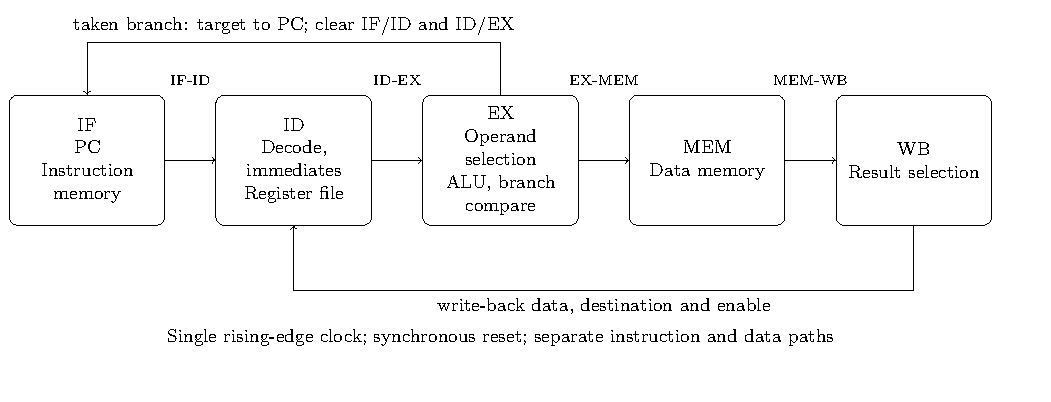
\includegraphics[width=\textwidth]{../diagrams/block.pdf}
\caption{Base datapath showing stage registers, the write-back path, and branch redirection. Forwarding feeds the EX operands. The interlock holds IF and ID and inserts a bubble into EX.}
\label{fig:block}
\end{figure*}

\begin{table}[t]
\caption{Decode control bits}
\label{tab:ctrl}
\centering\small
\begin{tabular}{lccccccc}\hline
 & RW & MR & MW & Imm & Sub & Br & NE\\\hline
ADD  &1&0&0&0&0&0&0\\
SUB  &1&0&0&0&1&0&0\\
ADDI &1&0&0&1&0&0&0\\
LW   &1&1&0&1&0&0&0\\
SW   &0&0&1&1&0&0&0\\
BEQ  &0&0&0&0&0&1&0\\
BNE  &0&0&0&0&0&1&1\\\hline
\end{tabular}
\par\smallskip\footnotesize RW: register write. MR/MW: memory read/write. Imm: use the immediate as ALU operand B. Sub: subtract. Br: branch. NE: compare for inequality.
\end{table}

Table~\ref{tab:ctrl} lists the control bits. The load bit also selects memory data in WB. Register and memory writes require a valid instruction. Each branch compares both source operands and adds the signed offset to its saved PC. On a taken branch, EX directs IF to the target and clears IF/ID and ID/EX at the next edge. The branch itself advances to MEM. The instruction in ID and the sequential fetch are discarded, with a cost of two slots.

\begin{figure*}[t]
\centering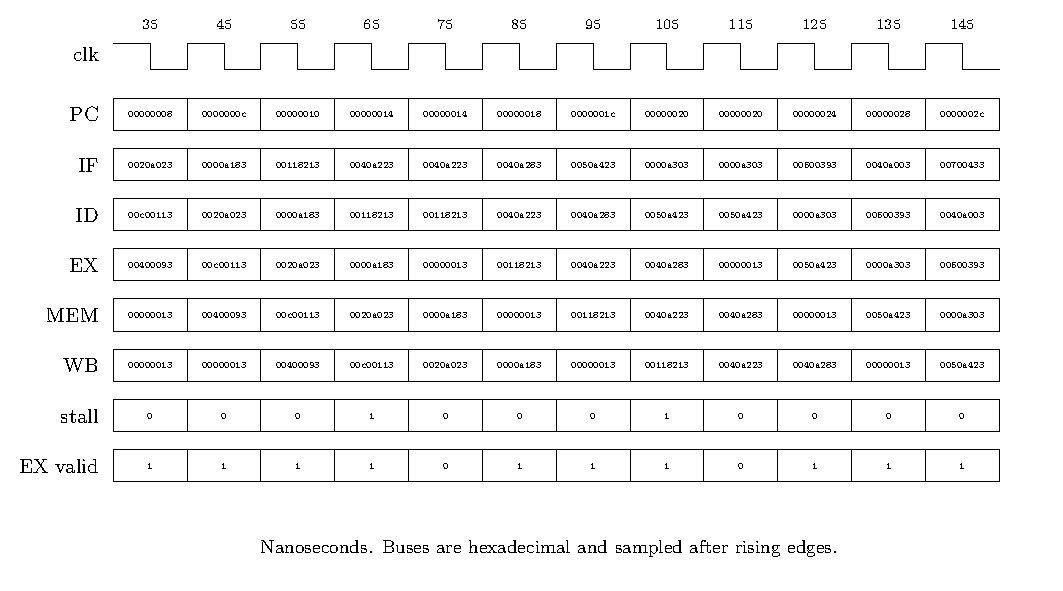
\includegraphics[width=\textwidth]{../waveforms/load_use.pdf}
\caption{Load-use VCD from the pipeline run. At 65 ns the load for x3 is in EX and its dependent ADDI is in ID. The edge at 75 ns holds the PC and ID and inserts a bubble. At 85 ns the ADDI enters EX as the load reaches WB. The visible second stall has a store-data dependency.}
\label{fig:wave}
\end{figure*}

\subsection{Forwarding and the load-use interlock}
Each EX source first checks for a valid, nonzero destination in EX/MEM. A matching ALU result there takes priority over one in MEM/WB because EX/MEM holds the more recent instruction. An EX/MEM load cannot forward its effective address as a register result. Its read data becomes available in MEM/WB, where WB supplies it to the consumer. The register file also passes a same-edge WB write to an ID read of that destination.

Forwarded A can supply an arithmetic input or the base address for a load or store. Forwarded B can supply the second register operand, a branch comparison or the value a store writes. A store uses its immediate to calculate the address even when forwarding supplies the value to write.

The interlock checks a valid load in EX against a valid consumer in ID. Every supported instruction uses rs1. Only ADD, SUB, SW, BEQ and BNE use rs2, so an immediate that happens to share those bit positions cannot cause a false stall. The check also ignores loads to x0. On a match, the next edge holds the PC and IF/ID and inserts an invalid entry into ID/EX. The load advances. One cycle later the consumer enters EX and receives the value from WB. Reset and taken-branch redirection have priority over a hold.

\subsection{Single-cycle baseline}
The baseline uses the same decoder, ALU, memory modules and write-back selection. It has no interstage registers, so the current instruction reads register state left by preceding edges and writes its own result at the end of the cycle. Its register file disables same-cycle write-through. Enabling it on this datapath could feed an instruction's result back into its own source. A taken branch selects the target for the next fetch within the current cycle.

\section{Results and Discussion}
\subsection{Simulation and retirement checks}
We used Icarus Verilog for RTL simulation~\cite{icarus}. The ALU, register file and decoder passed 59 unit cases. We also checked 22 pipeline runs and three baseline runs. The pipeline suite includes four Phase I programs, three directed edge cases and twelve repeatable unpadded random programs. Both cores ran the three benchmarks assembled with GNU RISC-V binutils. At each retirement the software model checks the PC, instruction and register write. The testbenches check the expected state of all 32 registers and 64 data words.

The pipeline bench checks for simultaneous occupancy of all five stages at different instruction addresses. It also checks that a taken branch reaches the target and clears the two younger entries, and that a load-use stall holds fetch and decode while creating an EX bubble. In temporary copies, disabling one EX forwarding input or disabling the load interlock caused register-state failures. The complete suite passed from a fresh copy, and both RTL tops passed Verilator lint.

The bench counts an instruction when it completes WB in the pipeline or reaches the end of its only cycle in the baseline. Stores, branches and explicit NOPs count. Bubbles and flushed instructions never retire. Each bench counts cycles from the first rising edge after reset release through retirement of the instruction at its configured stop address. The core continues fetching after that address.

\subsection{Benchmark cycle counts}
Table~\ref{tab:bench} uses identical binaries and stop addresses on both cores. CPI is cycles divided by retired instructions. IPC uses the reciprocal. The single-cycle results are 1.000 CPI and 1.000 IPC throughout. Each pipeline run satisfies
\[
C = N + 4 + S + 2T ,
\]
where $N$ is the number of retirements, $S$ is the number of stalls and $T$ is the number of taken branches. The four-cycle term is pipeline fill before the first retirement.

\begin{table}[!t]
\caption{Cycle counts and pipeline CPI/IPC from RTL simulation. Both cores retire the same instruction sequence.}
\label{tab:bench}\centering\footnotesize
\setlength{\tabcolsep}{2.3pt}
\begin{tabular}{lrrrrrrr}\hline
 & & \multicolumn{2}{c}{Cycles} & & & \multicolumn{2}{c}{Pipeline}\\
Benchmark & Ret. & Single & Pipe & Stalls & Taken & CPI & IPC\\\hline
ALU chain   &  7 &  7 & 11 & 0 & 0 & 1.571 & 0.636\\
Load use    & 14 & 14 & 21 & 3 & 0 & 1.500 & 0.667\\
Branch loop & 18 & 18 & 31 & 1 & 4 & 1.722 & 0.581\\\hline
\end{tabular}
\end{table}

The ALU chain runs without stalls, even with back-to-back writes to x1. The load benchmark stalls once for each of three immediate load dependencies. Fig.~\ref{fig:wave} shows a load feeding arithmetic and another feeding a store. An independent ADDI and a load to x0 cause no stalls. The loop takes three backward branches and one forward branch after a load. Clearing the wrong path skips a register write and a store. These small benchmarks isolate the cycle costs of the dependencies and branches they exercise.

\subsection{Synthesis and FPGA timing}
We synthesized the two top modules in Yosys 0.71+77, then placed and routed them with nextpnr-ice40 (revision 15b77f5f)~\cite{fpga}. We used the branch-loop ROM, the same fetch and retirement ports, and one iCE40HX8K CT256 target for both cores. The placer used seed~1 and a 12 MHz clock target. The FPGA script saves the netlists, tool logs and timing JSON.

\begin{table}[t]
\caption{Post-route utilization and clock estimates}
\label{tab:fpga}\centering
\begin{tabular}{lrr}\hline
Metric & Single-cycle & Pipeline\\\hline
Logic cells & 5,310 & 5,843\\
Block RAMs & 0 & 0\\
I/O pins & 169 & 169\\
Critical period (ns) & 32.93 & 23.40\\
Maximum clock (MHz) & 30.37 & 42.74\\\hline
\end{tabular}
\end{table}

Both cores met the 12 MHz internal target. The pipeline used 10.0\% more logic cells. Combinational reads and synchronous clearing of writable state map the local memories to logic in this build. The fetch and retirement outputs account for much of the package I/O. In zero-delay simulation, both mapped netlists matched their RTL retirement trace for the branch loop. The companion FPGA synthesis and timing report gives the mapped resource counts and critical paths.

At the estimated maximum clocks, the branch loop would take 0.593 microseconds on the single-cycle core ($18/30.37$) and 0.725 microseconds on the pipeline ($31/42.74$). That is 30.37 and 24.82 million retirements per second, respectively, over this run. At the shared 12 MHz target, runtime is proportional to cycle count. These timing estimates apply to the routed branch-loop image with automatic pin placement. Board-level I/O timing and physical operation remain unmeasured.

\section{Individual Contributions}
The module ownership below follows the repository contributions. Aryan Kinha coordinated integration and verification as team lead.

\begin{center}\footnotesize
\begin{tabular}{p{0.36\columnwidth}p{0.54\columnwidth}}\hline
Member & Module ownership\\\hline
Aryan Kinha\newline 2401020013 & Top-level integration, tests and report.\\
Preetish Ubhrani\newline 2401020050 & Execute stage, ALU and branch comparison.\\
Divyanshu Singh\newline 2401010161 & Decode, control, immediates and register file.\\
Jatin Verma\newline 2401010200 & Data memory, MEM/WB and write-back.\\
Jatin Kumar Singh\newline 2401010199 & Fetch, PC, instruction memory and IF/ID.\\\hline
\end{tabular}
\end{center}

\section{Conclusion}
The five-stage core ran all three benchmarks without software padding. Forwarding handled adjacent ALU dependencies, and each immediate load dependency cost one cycle. The pipeline's estimated clock period fell from 32.93 ns to 23.40 ns on the FPGA target. For the branch loop, the increase from 18 to 31 cycles outweighed that shorter period.

\begin{thebibliography}{10}
\bibitem{isa} RISC-V International, \emph{The RISC-V Instruction Set Manual, Volume I: Unprivileged Architecture}, ver. 20240411, 2024. [Online]. Available: \url{https://docs.riscv.org/reference/isa/v20240411/unpriv/unpriv-index.html}
\bibitem{patterson} D. A. Patterson and J. L. Hennessy, \emph{Computer Organization and Design RISC-V Edition: The Hardware Software Interface}, 2nd ed. Morgan Kaufmann, 2020. [Online]. Available: \url{https://shop.elsevier.com/books/computer-organization-and-design-risc-v-edition/patterson/978-0-12-820331-6}
\bibitem{harris} S. L. Harris and D. Harris, \emph{Digital Design and Computer Architecture, RISC-V Edition}. Morgan Kaufmann, 2021. [Online]. Available: \url{https://pages.hmc.edu/harris/ddca/ddcarv.html}
\bibitem{pico} YosysHQ, ``PicoRV32: A size-optimized RISC-V CPU,'' source repository. Accessed: Nov. 13, 2026. [Online]. Available: \url{https://github.com/YosysHQ/picorv32}
\bibitem{ibex} lowRISC, ``Ibex RISC-V core,'' source repository. Accessed: Nov. 13, 2026. [Online]. Available: \url{https://github.com/lowRISC/ibex}
\bibitem{vex} SpinalHDL, ``VexRiscv,'' source repository. Accessed: Nov. 13, 2026. [Online]. Available: \url{https://github.com/SpinalHDL/VexRiscv}
\bibitem{cv} OpenHW Group, ``CORE-V CV32E40P RISC-V IP,'' source repository. Accessed: Nov. 13, 2026. [Online]. Available: \url{https://github.com/openhwfoundation/cv32e40p}
\bibitem{icarus} Icarus Verilog contributors, ``Icarus Verilog documentation.'' Accessed: Nov. 13, 2026. [Online]. Available: \url{https://steveicarus.github.io/iverilog/}
\bibitem{comparison} Ario2006, ``risc-5-processor,'' source repository, revision 6a9a36c. Accessed: Nov. 15, 2026. [Online]. Available: \url{https://github.com/Ario2006/risc-5-processor/tree/6a9a36c8434b05719c9045d768cd16f4a9162eca}
\ifdefined\phaseTwoReport
\bibitem{fpga} D. Shah, E. Hung, C. Wolf, S. Bazanski, D. Gisselquist, and M. Milanovi\'{c}, \textquotedblleft Yosys+nextpnr: An open source framework from Verilog to bitstream for commercial FPGAs,\textquotedblright\ in \emph{Proc. IEEE 27th Annu. Int. Symp. Field-Programmable Custom Computing Machines (FCCM)}, 2019, doi: 10.1109/FCCM.2019.00010.
\fi
\end{thebibliography}

\end{document}
